\section{Motivation}
% 1.5 pages
Serverless Computing is a computing paradigm which alleviates application developers from deployment considerations to an unprecedented level. % cite general serverless
In traditional, and even in modern containerized computing environments, developers are required to explicitly specify how their application should be deployed, thus requiring a great deal of effort and high level of competency. %todo cite this
With the introduction of edge computing, the adaptation of serverless platforms was proposed as a means to abstract the additional complexity arising from edge computing, allowing one to make use of the advantages and new possibilities of edge computing more readily \cite{nasticServerlessRealTimeData2017}\cite{gliksonDevicelessEdgeComputing2017}.
Edge Computing does, however, have it's own range of specific challenges that need to be overcome to make use of it effectively \cite{shiEdgeComputingVisionChallenges2016}.

Serverless platforms typically utilize existing technologies to provide their functionality. Most of all they rely on containerization techniques, and as a result the techniques used to manage large scale container deployments.
For this reason popular serverless platforms such as kubeless\cite{kubeless} and OpenFaaS\cite{openfaas} are built on top of Kubernetes, the far and away most common container orchestration platform.
Neither these platforms, nor the underlying container orchestration technology, are by default suited for the unique conditions posed by edge computing, in particular increased heterogeneity in both network structure and compute capability.
OpenFaaS has been adapted as a serverless system by Rausch et al. with a focus on optimized container scheduling \cite{skippy}.
While function placement has been studied more extensively, efficient processing of network bound workloads, meaning workloads where network transfers are the dominant part of the overall response time, remains a challenge. For serverless frameworks like OpenFaaS, one of the likely causes is the centralized architecture of it and the underlying container orchestration framework, as outlined by Rausch et al.\cite{skippy}.
This centralization leads to the system routing requests in a highly inefficient manner, thus likely causing the relatively poor response times of network bound workloads. A potential solution outlined by Rausch et al. is to distribute the ingress points throughout the cluster, including to the edge\cite{skippy}.
The ingress points first accept the request and forward it to a function replicas, thus acting as a load balancer for incoming requests.

\begin{figure}
    \centering
    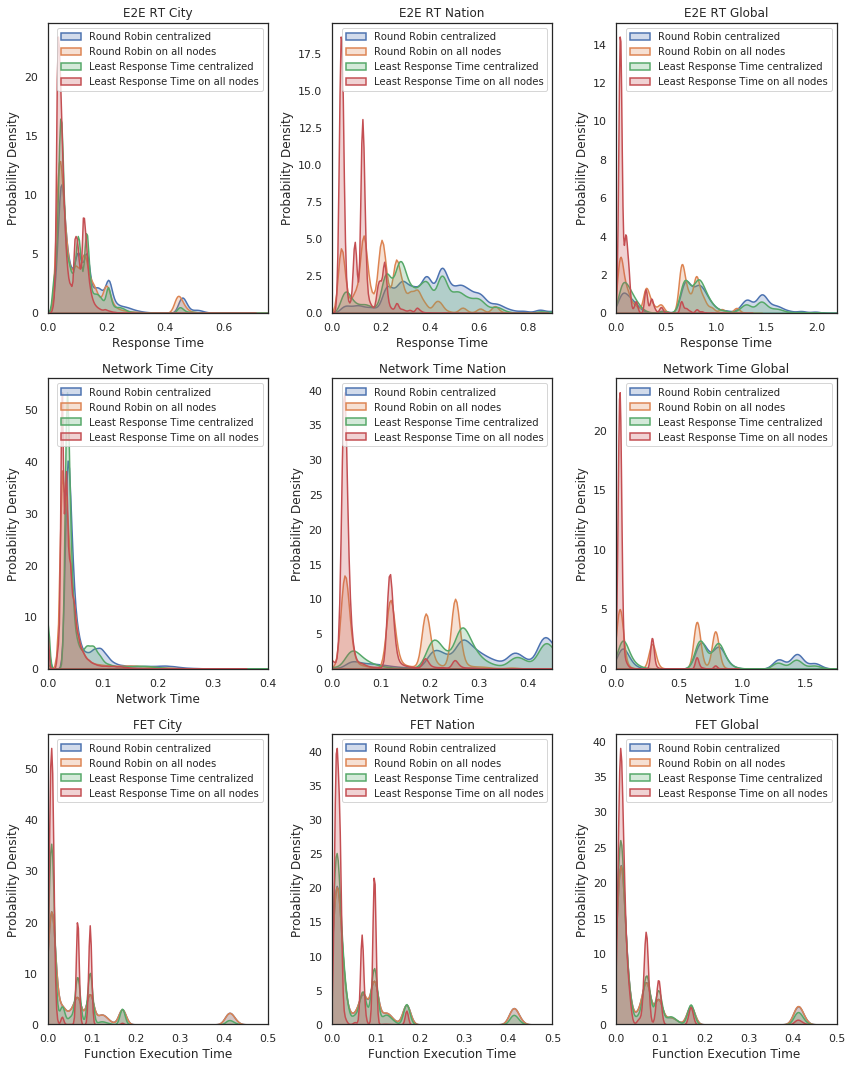
\includegraphics[width=\linewidth]{graphics/graphs/initial_eval_pdfs_3x3.png}
    \caption{Kernel Density Estimate of a single experiment run. Shown data can be interpreted as probability density functions. Data is visualized for \gls{trt}, \gls{fet} and the time incurred through network transfers.}
    \label{fig:initial_eval_pdfs}
\end{figure}

Before developing an approach to the range of engineering challenges such a solution requires we decided to perform a preliminary analysis in order to determine whether distributed load balancers for the serverless system are a viable solution at all, and if so by how much the performance of network bound workloads can be improved.
To this end we used Faas-Sim\cite{faas-sim-github},
a serverless edge computing simulator built to emulate the core concepts of OpenFaaS and Kubernetes. Building on the work done by Philipp Raith \cite{philipp-da},
we extended the simulator with a more realistic and adaptable method for load balancing, allowing different load balancing techniques to be employed, and taking into account function placement and network conditions when simulating requests.%
This preliminary analysis shows an improvement in mean response time of between 81.3\% and 606.9\%, depending on the scenario. Fig \ref{fig:initial_eval_pdfs}
shows the fitted probability density functions of the overall response time, function execution time, and network transfer time in different scenarios. From this data we can see that:
\begin{enumerate}
    \item distribution of load balancers alone is insufficient to improve performance,
    \item more sophisticated load balancing methods are required to make use of network proximity, and
    \item sophisticated load balancing methods can, in addition to improving network induced delay, reduce function execution time.
    \iitem The location of load balancers has a significant impact on performance, making the effective placement of load balancers important
\end{enumerate}
Based on these results we believe that it is worthwhile to explore this area further, and in more detail than the preliminary evaluation could.

